\chapter{Hardwareaufbau}

Im Rahmen des Projektes, wurde der Roboter durch einen externen Hardwareaufbau erweitert. Die prinzipielle Schnittstelle zwischen
Roboter und Steckbrett wurde unter Verwendung eines I$^2$C-Expanders realisiert.

\begin{figure}[h]
	\centering
		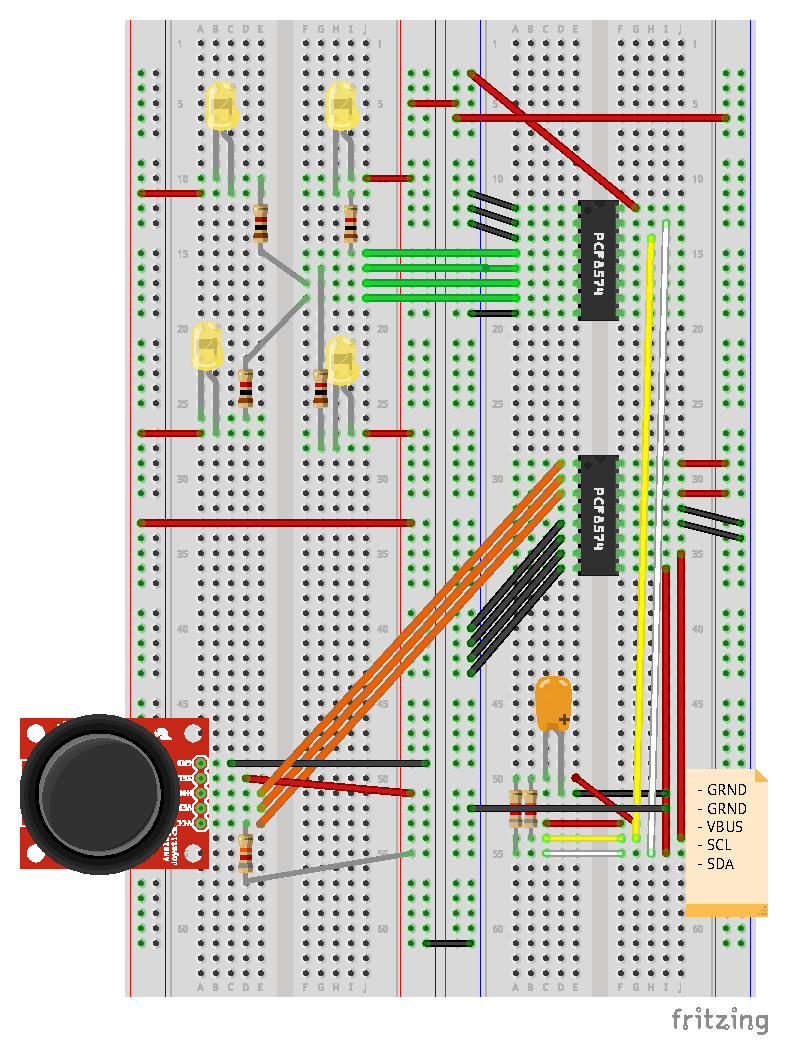
\includegraphics[page=1,width=0.5\textwidth]{Dokumente/Schaltplan.pdf}
	\caption{Hardwareaufbau auf Steckbrett}
	\label{fig:hardwareaufbau}
\end{figure}

In Abbildung \ref{fig:hardwareaufbau} ist die finale Erweiterung dargestellt. Folgende Bauteile wurden hierfür verwendet:

\begin{itemize}
	\item 2 PCF8574 Schnittstellen-IC
	\item 4 LEDs
	\item Joystick
\end{itemize}
\newpage
Der Roboter kann nun über ein Verbindungskabel an das Steckbrett angebunden werden. Hierfür teilen sich die zwei ICs einen I$^2$C-Bus.
Aus Gründen der besseren Übersicht, wurden die LEDs sowie der Joystick an jeweils eigene ICs angeschlossen.\newline \newline
Die LEDs sind, wie in Abbildung \ref{fig:hardwareaufbau} gezeigt, an den oberen IC angeschlossen. Es werden vier der sieben Digital-IO Pins
verwendet.\newline \newline
Der Joystick ist, wie in Abbildung \ref{fig:hardwareaufbau} gezeigt, an den unteren IC angeschlossen. Es werden alle der drei Analogen-IO Pins verwendet.